\section{Constant Coefficient Homogeneous Equations}

\noindent
If $a,b$, and $c$ are real constants and $a\ne0$, then
$$
ay''+by'+cy=F(x)
$$
 is said to be a {\color{blue}\it constant coefficient
 equation}.
In this section we  consider the homogeneous constant
coefficient equation
\begin{equation} \label{eq:5.2.1}
ay''+by'+cy=0.
\end{equation}
As we'll see, all solutions of \eqref{eq:5.2.1} are defined on
$(-\infty,\infty)$.  This being the case, we'll omit references to the
interval on which solutions are defined, or on which a given set of
solutions is a fundamental set, etc., since the interval will always
be $(-\infty,\infty)$.

The key to solving \eqref{eq:5.2.1} is  that if
 $y=e^{rx}$ where $r$ is a constant  then the left side of
\eqref{eq:5.2.1} is a  multiple of $e^{rx}$;   thus, if $y=e^{rx}$
 then $y'=re^{rx}$ and $y''=r^2e^{rx}$, so
\begin{equation} \label{eq:5.2.2}
ay''+by'+cy=ar^2e^{rx}+bre^{rx}+ce^{rx}=(ar^2+br+c)e^{rx}.
\end{equation}
The quadratic polynomial
$$
p(r)=ar^2+br+c
$$
is  the {\color{blue}\it characteristic polynomial\/} of \eqref{eq:5.2.1}, and
$p(r)=0$
is  the {\color{blue}\it characteristic equation\/}.
From \eqref{eq:5.2.2} we can see that $y=e^{rx}$ is a solution of
\eqref{eq:5.2.1}  if and only if $p(r)=0$.

The roots of  the  characteristic equation are given by the quadratic
formula
\begin{equation} \label{eq:5.2.3}
r={-b\pm\sqrt{b^2-4ac}\over2a}.
\end{equation}
We consider three cases:
\begin{description}
\item{\sc Case 1.} $b^2-4ac>0$, so the characteristic equation has two
distinct real roots.
\item{\sc Case 2.} $b^2-4ac=0$, so the characteristic equation has a
repeated real root.
\item{\sc Case 3.} $b^2-4ac<0$, so the characteristic equation has
complex roots.
\end{description}
In each case we'll start with an example.

\boxit{Case 1: Distinct Real Roots}

\noindent
\begin{example}\label{example:5.2.1}\rm  \mbox{} \newline
\begin{alist}
\item %(a)
Find the general solution of
\begin{equation} \label{eq:5.2.4}
y''+6y'+5y=0.
\end{equation}

\item %(b)
Solve the initial value problem
\begin{equation} \label{eq:5.2.5}
y''+6y'+5y=0, \quad   y(0)=3,\;  y'(0)=-1.
\end{equation}
\end{alist}
\end{example}

\solutionpart{a}   The characteristic
polynomial of
 \eqref{eq:5.2.4} is
$$
p(r)=r^2+6r+5=(r+1)(r+5).
$$
Since $p(-1)=p(-5)=0$,  $y_1=e^{-x}$ and $y_2=e^{-5x}$
are solutions of \eqref{eq:5.2.4}. Since $y_2/y_1=e^{-4x}$  is
nonconstant, \ref{thmtype:5.1.6} implies that the general solution
of \eqref{eq:5.2.4} is
\begin{equation} \label{eq:5.2.6}
y=c_1e^{-x}+c_2e^{-5x}.
\end{equation}

\solutionpart{b} We  must determine $c_1$ and $c_2$
in  \eqref{eq:5.2.6} so that $y$ satisfies the initial conditions in
 \eqref{eq:5.2.5}. Differentiating  \eqref{eq:5.2.6} yields
\begin{equation} \label{eq:5.2.7}
y'=-c_1e^{-x}-5c_2e^{-5x}.
\end{equation}
Imposing the initial conditions $y(0)=3,\, y'(0)=-1$ in \eqref{eq:5.2.6}
and \eqref{eq:5.2.7} yields
$$\begin{array}{rcr}
\phantom{-}c_1+\phantom{5}c_2 & = & 3\phantom{.}\\
-c_1-5c_2 & = & -1.
\end{array}$$
 The solution of this system is $c_1=7/2,c_2=-1/2$.  Therefore
the solution of  \eqref{eq:5.2.5} is
$$
y={7\over2}e^{-x}-{1\over2}e^{-5x}.
$$
 Figure~\ref{figure:5.2.1} is a graph
of this solution.

\begin{figure}[tbp]
  \centering
  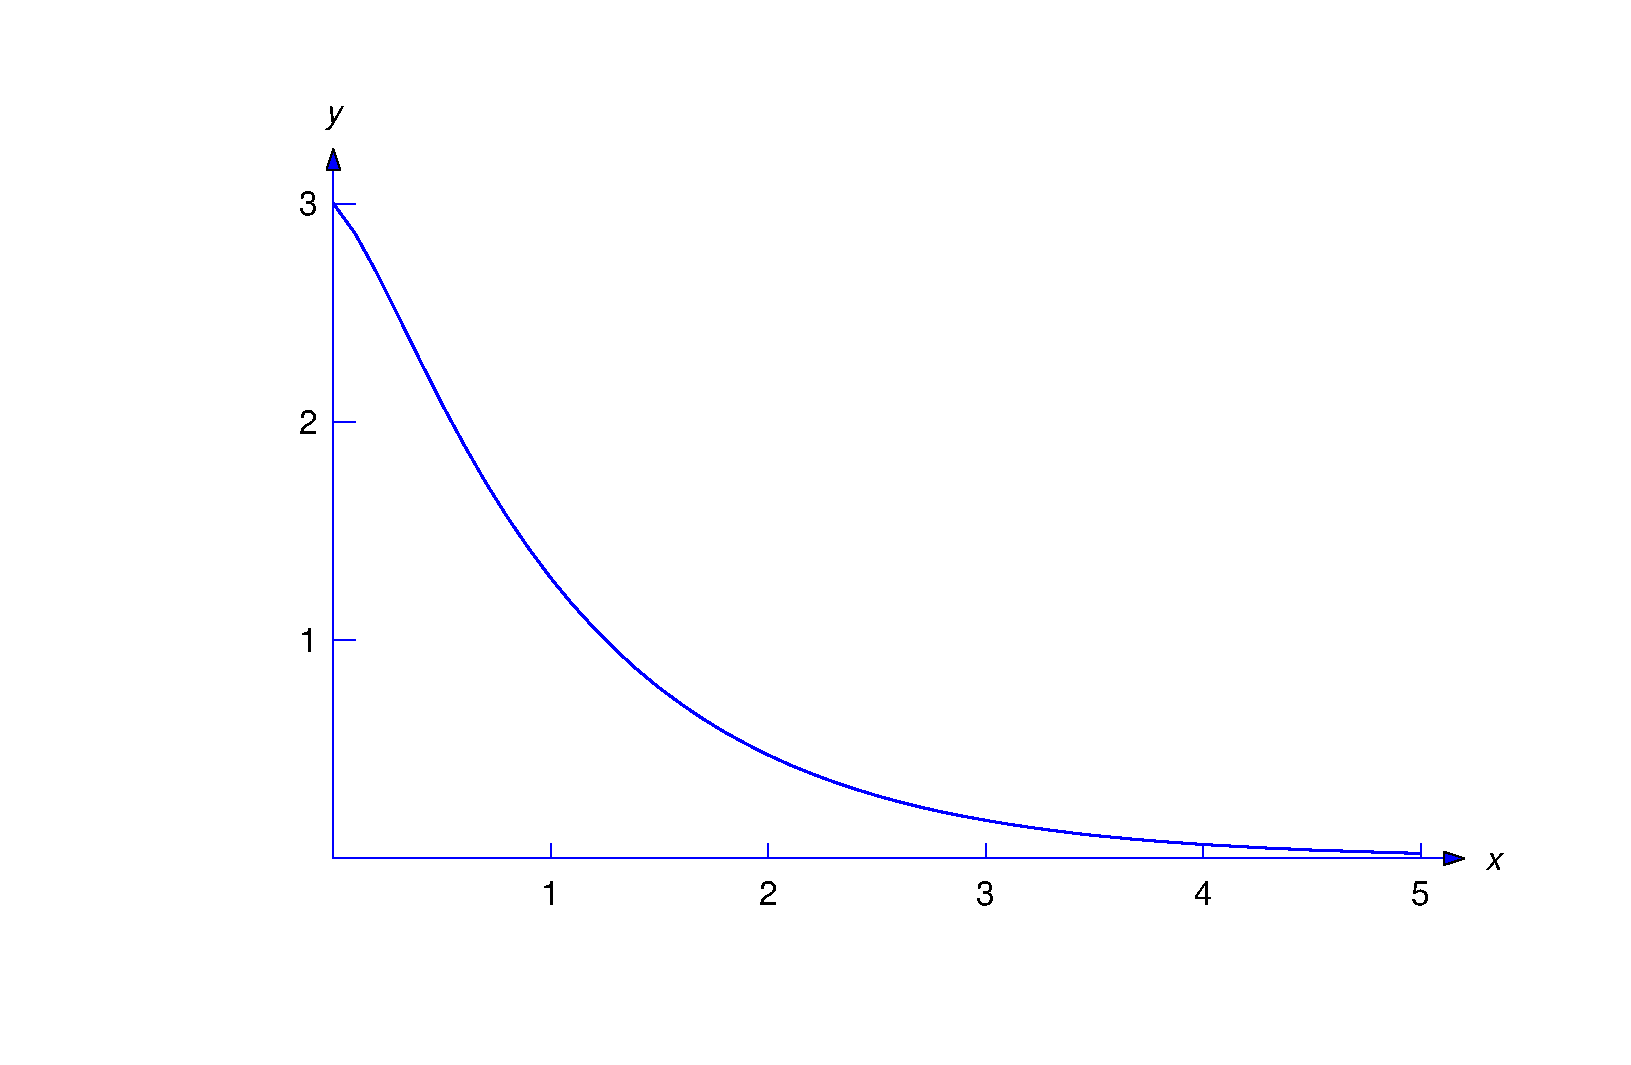
\includegraphics[bb=-78 148 689 643,width=5.67in,height=3.66in,keepaspectratio]{fig050201}
\color{blue}
  \caption{$y=\dst{{7\over2}e^{-x}-{1\over2}e^{-5x}}$ }
  \label{figure:5.2.1}
\end{figure}

If the characteristic equation has arbitrary distinct real roots
$r_1$ and $r_2$, then
$y_1=e^{r_1x}$ and $y_2=e^{r_2x}$  are  solutions of $ay''+by'+cy=0$.
Since $y_2/y_1=e^{(r_2-r_1)x}$ is nonconstant, Theorem~\ref{thmtype:5.1.6}
 implies that  $\{y_1,y_2\}$ is a fundamental
set of solutions of $ay''+by'+cy=0$.

\newpage
\boxit{Case 2: A Repeated Real Root}

\noindent
\begin{example}\label{example:5.2.2}\rm \mbox{}\newline
\begin{alist}
\item %(a)
Find the general solution of
\begin{equation} \label{eq:5.2.8}
y''+6y'+9y=0.
\end{equation}

\item %(b)
Solve the initial value problem
\begin{equation} \label{eq:5.2.9}
y''+6y'+9y=0, \quad   y(0)=3,\;  y'(0)=-1.
\end{equation}
\end{alist}
\end{example}

\solutionpart{a}   The characteristic polynomial of
 \eqref{eq:5.2.8} is
$$
p(r)=r^2+6r+9=(r+3)^2,
$$
so the characteristic equation has the repeated real root $r_1=-3$.
Therefore $y_1=e^{-3x}$ is a solution of \eqref{eq:5.2.8}. Since the
characteristic equation has no other roots, \eqref{eq:5.2.8}
has no other  solutions of the form $e^{rx}$.
 We  look for  solutions of the form
$y=uy_1=ue^{-3x}$,
where $u$ is a function that we'll now
determine.
(This should remind you of the method of variation of parameters
used in Section~2.1 to solve the nonhomogeneous
equation $y'+p(x)y=f(x)$, given a solution $y_1$ of the complementary
equation $y'+p(x)y=0$.  It's also a special case of a method called
{\color{blue}\it reduction of order\/} that we'll study in Section~5.6.
For other ways to obtain a second solution of \eqref{eq:5.2.8} that's
not a multiple of $e^{-3x}$, see
Exercises~5.1.~\hspace*{-3pt}\ref{exer:5.1.9},
5.1.~\hspace*{-3pt}\ref{exer:5.1.12}, and \ref{exer:5.2.33}.

If $y=ue^{-3x}$, then
$$
y'=u'e^{-3x}-3ue^{-3x}\mbox{\quad and \quad}
y''=u''e^{-3x}-6u'e^{-3x}+9ue^{-3x},
$$
so
\begin{eqnarray*}
y''+6y'+9y&=&e^{-3x}\left[(u''-6u'+9u)+6(u'-3u)+9u\right]\\
&=&e^{-3x}\left[u''-(6-6)u'+(9-18+9)u\right]=u''e^{-3x}.
\end{eqnarray*}
Therefore $y=ue^{-3x}$ is a solution of \eqref{eq:5.2.8} if and only if
$u''=0$, which is equivalent to $u=c_1+c_2x$, where $c_1$ and $c_2$
are constants. Therefore any function of the form
\begin{equation} \label{eq:5.2.10}
y=e^{-3x}(c_1+c_2x)
\end{equation}
is  a solution of \eqref{eq:5.2.8}.
Letting $c_1=1$ and $c_2=0$  yields the solution
 $y_1=e^{-3x}$ that we already knew. Letting $c_1=0$ and $c_2=1$
yields the second solution $y_2=xe^{-3x}$. Since
$y_2/y_1=x$
is nonconstant, \ref{thmtype:5.1.6} implies that   $\{y_1,y_2\}$ is
fundamental set of solutions of \eqref{eq:5.2.8}, and \eqref{eq:5.2.10}
is the general solution.

\solutionpart{b}  Differentiating   \eqref{eq:5.2.10} yields
\begin{equation} \label{eq:5.2.11}
y'=-3e^{-3x}(c_1+c_2x)+c_2e^{-3x}.
\end{equation}
Imposing the initial conditions $y(0)=3,\, y'(0)=-1$ in \eqref{eq:5.2.10}
and \eqref{eq:5.2.11} yields $c_1=3$ and $-3c_1+c_2=-1$, so
$c_2=8$. Therefore the solution of \eqref{eq:5.2.9} is
$$
y=e^{-3x}(3+8x).
$$
Figure~\ref{figure:5.2.2} is a graph of this solution.

\enlargethispage{2in}

\begin{figure}[H]
  \centering
  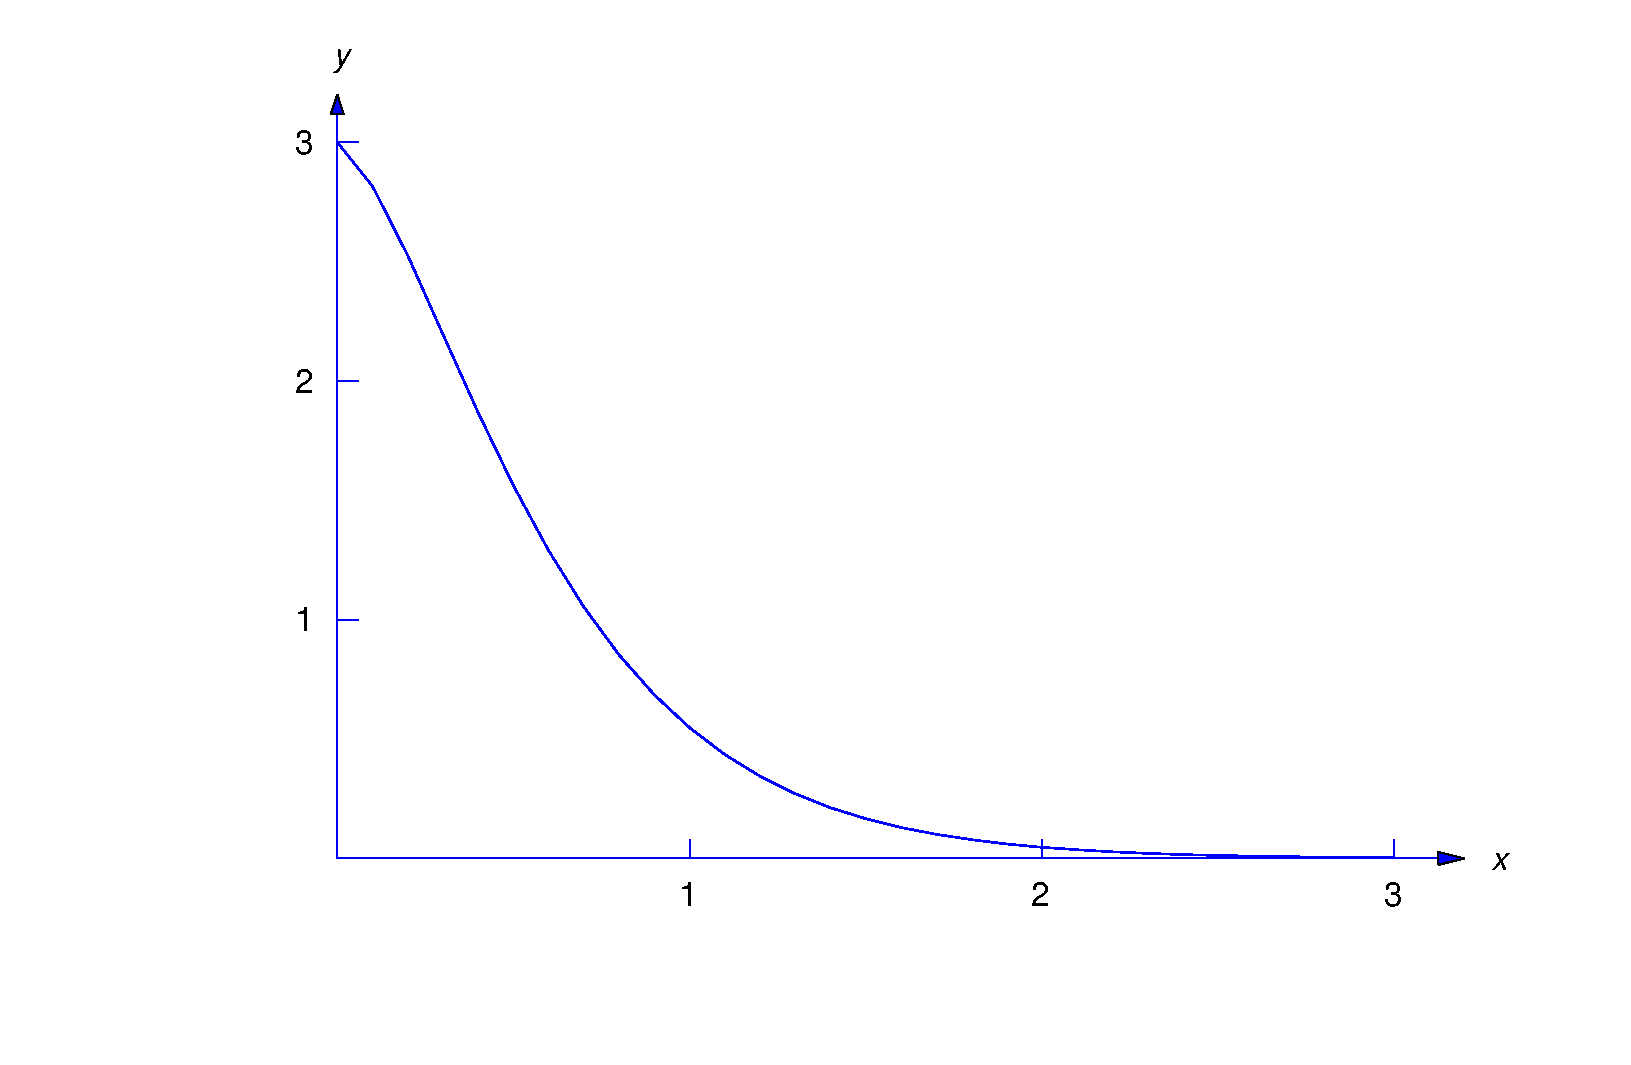
\includegraphics[bb=-78 148 689 643,width=5.67in,height=3.66in,keepaspectratio]{fig050202}
\color{blue}
\vspace*{-10pt}
  \caption{$y=e^{-3x}(3+8x)$}
  \label{figure:5.2.2}
\end{figure}

\newpage
If the characteristic equation of $ay''+by'+cy=0$
has an arbitrary repeated root $r_1$,  the
characteristic polynomial must be
$$
p(r)=a(r-r_1)^2=a(r^2-2r_1r+r_1^2).
$$
Therefore
$$
ar^2+br+c=ar^2-(2ar_1)r+ar_1^2,
$$
which implies that $b=-2ar_1$ and $c=ar_1^2$.
Therefore
 $ay''+by'+cy=0$ can be written as
$a(y''-2r_1y'+r_1^2y)=0$. Since $a\ne0$ this equation has the same
solutions as
\begin{equation} \label{eq:5.2.12}
y''-2r_1y'+r_1^2y=0.
\end{equation}

Since $p(r_1)=0$, t $y_1=e^{r_1x}$ is a solution of
$ay''+by'+cy=0$, and therefore of \eqref{eq:5.2.12}. Proceeding as in
Example~\ref{example:5.2.2}, we look for other solutions of \eqref{eq:5.2.12}
of the form $y=ue^{r_1x}$; then
$$
y'=u'e^{r_1x}+rue^{r_1x}\mbox{\quad and \quad}
y''=u''e^{r_1x}+2r_1u'e^{r_1x}+r_1^2ue^{r_1x},
$$
so
\begin{eqnarray*}
y''-2r_1y'+r_1^2y&=&e^{rx}\left[(u''+2r_1u'+r_1^2u)-
2r_1(u'+r_1u)+r_1^2u\right]\\
&=&e^{r_1x}\left[u''+(2r_1-2r_1)u'+(r_1^2-2r_1^2+r_1^2)u\right]=u''e^{r_1x}.
\end{eqnarray*}
Therefore $y=ue^{r_1x}$ is a solution of \eqref{eq:5.2.12} if and only if
$u''=0$, which is equivalent to $u=c_1+c_2x$, where $c_1$ and $c_2$
are constants. Hence, any function of the form
\begin{equation} \label{eq:5.2.13}
y=e^{r_1x}(c_1+c_2x)
\end{equation}
is  a solution of \eqref{eq:5.2.12}.
Letting $c_1=1$ and $c_2=0$ here yields the solution
 $y_1=e^{r_1x}$ that we already knew. Letting $c_1=0$ and $c_2=1$
yields the second solution $y_2=xe^{r_1x}$. Since
$y_2/y_1=x$
is nonconstant, \ref{thmtype:5.1.6} implies that   $\{y_1,y_2\}$ is
a fundamental set of solutions of \eqref{eq:5.2.12}, and \eqref{eq:5.2.13}
is the general solution.

\boxit{Case 3: Complex Conjugate Roots}

\vspace*{-20pt}
\noindent
\begin{example}\label{example:5.2.3}\rm \mbox{}\newline
\begin{alist}
\item %(a)
Find the general solution of
\begin{equation} \label{eq:5.2.14}
y''+4y'+13y=0.
\end{equation}

\item %(b)
Solve the initial value problem
\begin{equation} \label{eq:5.2.15}
y''+4y'+13y=0, \quad   y(0)=2,\;  y'(0)=-3.
\end{equation}
\end{alist}
\end{example}

\solutionpart{a}  The characteristic
polynomial of
 \eqref{eq:5.2.14} is
$$
p(r)=r^2+4r+13=r^2+4r+4+9=(r+2)^2+9.
$$
The roots of the characteristic equation are $r_1=-2+3i$ and
$r_2=-2-3i$. By analogy with Case~1, it's reasonable to expect that
$e^{(-2+3i)x}$ and $e^{(-2-3i)x}$ are solutions of \eqref{eq:5.2.14}. This
is true (see Exercise~\ref{exer:5.2.34});     however, there are
difficulties here, since you are probably not familiar with
exponential functions with complex arguments, and even if you are, it's
 inconvenient to work with them, since they are complex--valued. We'll
 take a simpler approach, which we motivate as follows: the
exponential notation suggests that
$$
e^{(-2+3i)x}=e^{-2x}e^{3ix}\mbox{\quad and \quad}
e^{(-2-3i)x}=e^{-2x}e^{-3ix},
$$
so even though we haven't defined $e^{3ix}$ and $e^{-3ix}$, it's
reasonable to expect that every linear
combination of $e^{(-2+3i)x}$ and $e^{(-2-3i)x}$ can be written as
$y=ue^{-2x}$, where $u$ depends upon $x$. To determine $u$, we note
that if $y=ue^{-2x}$ then
$$
y'=u'e^{-2x}-2ue^{-2x}\mbox{\quad and \quad}
y''=u''e^{-2x}-4u'e^{-2x}+4ue^{-2x},
$$
so
\begin{eqnarray*}
y''+4y'+13y&=&e^{-2x}\left[(u''-4u'+4u)+4(u'-2u)+13u\right]\\
&=&e^{-2x}\left[u''-(4-4)u'+(4-8+13)u\right]=e^{-2x}(u''+9u).
\end{eqnarray*}
Therefore $y=ue^{-2x}$ is a solution of \eqref{eq:5.2.14} if and only if
$$
u''+9u=0.
$$
From Example~\ref{example:5.1.2}, the  general solution of this equation is
$$
u=c_1\cos 3x +c_2\sin 3x.
$$
 Therefore any function of the form
\begin{equation} \label{eq:5.2.16}
y=e^{-2x}(c_1\cos 3x+c_2\sin 3x)
\end{equation}
is  a solution of \eqref{eq:5.2.14}.
Letting $c_1=1$ and $c_2=0$  yields the solution
 $y_1=e^{-2x}\cos3x$. Letting $c_1=0$ and $c_2=1$
yields the second solution $y_2=e^{-2x}\sin3x$. Since
$y_2/y_1=\tan3x$
is nonconstant, \ref{thmtype:5.1.6} implies that   $\{y_1,y_2\}$ is
a fundamental set of solutions of \eqref{eq:5.2.14}, and \eqref{eq:5.2.16}
is the general solution.

\solutionpart{b}   Imposing the condition $y(0)=2$
in   \eqref{eq:5.2.16} shows that $c_1=2$.  Differentiating
\eqref{eq:5.2.16} yields
$$
y'=-2e^{-2x}(c_1\cos 3x+c_2\sin 3x) +3e^{-2x}(-c_1\sin 3x +c_2\cos 3x),
$$
and imposing the initial condition $y'(0)=-3$ here yields
$-3=-2c_1+3c_2=-4+3c_2$,
 so $c_2=1/3$. Therefore the solution of
\eqref{eq:5.2.15} is
$$
y=e^{-2x}(2\cos 3x+ {1\over3}\sin 3x).
$$
Figure~\ref{figure:5.2.3}  is a graph of this function. \bbox

      \begin{figure}[tbp]
  \centering
\color{blue}
  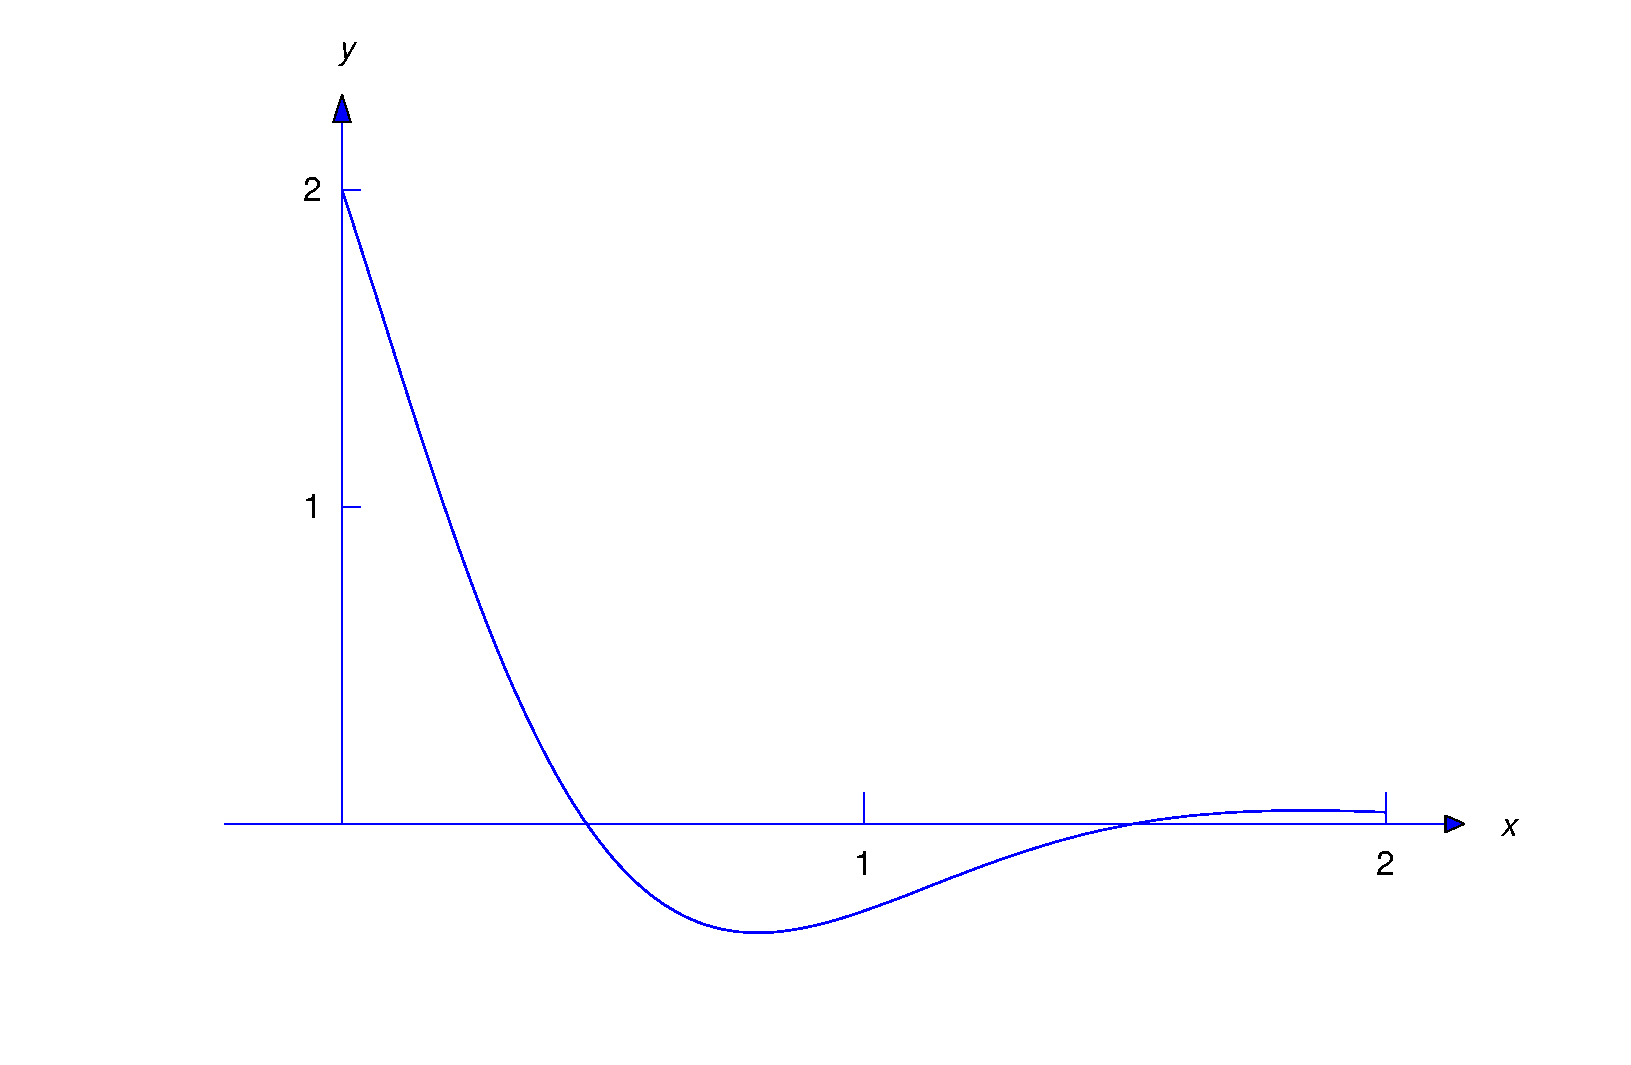
\includegraphics[bb=-78 148 689 643,width=5.67in,height=3.66in,keepaspectratio]{fig050203}
  \caption{$\dst{y=e^{-2x}(2\cos 3x+ {1\over3}\sin 3x)}$}
  \label{figure:5.2.3}
\end{figure}

Now suppose   the characteristic equation of $ay''+by'+cy=0$ has
arbitrary complex roots;   thus, $b^2-4ac<0$ and, from \eqref{eq:5.2.3},
the
roots are
$$
r_1 = {-b+i\sqrt{4ac-b^2}\over 2a},\quad r_2 =
{-b-i\sqrt{4ac-b^2}\over 2a},
$$
which we rewrite as
\begin{equation} \label{eq:5.2.17}
r_1=\lambda+i \omega,\quad r_2 = \lambda - i \omega,
\end{equation}
 with
$$
\lambda = -{b\over 2a},\quad \omega = {\sqrt{4ac-b^2}\over 2a}.
$$
Don't memorize these formulas. Just remember that $r_1$
and $r_2$ are of the form \eqref{eq:5.2.17},
where  $\lambda$ is an arbitrary real number and $\omega$
is   positive;
 $\lambda$ and $\omega$ are  the {\color{blue}\it real\/}
and {\color{blue}\it imaginary parts\/}, respectively, of $r_1$.
Similarly, $\lambda$ and $-\omega$ are the real and imaginary parts of
$r_2$. We say that $r_1$ and $r_2$ are {\color{blue}\it complex conjugates\/},
which means that they have the same real part and their imaginary
parts have the same absolute values, but opposite signs.

As in Example~\ref{example:5.2.3}, it's reasonable to
to expect that the solutions of $ay''+by'+cy=0$  are linear
combinations of
$e^{(\lambda+i\omega)x}$ and $e^{(\lambda-i\omega)x}$.
Again,  the exponential notation suggests that
$$
e^{(\lambda+i\omega)x}=e^{\lambda x}e^{i\omega x}\mbox{\quad and
\quad} e^{(\lambda-i\omega)x}=e^{\lambda x}e^{-i\omega x},
$$
so even though we haven't defined $e^{i\omega x}$ and
$e^{-i\omega x}$, it's reasonable to expect that every linear
combination of $e^{(\lambda+i\omega)x}$ and $e^{(\lambda-i\omega)x}$
can  be written as
$y=ue^{\lambda x}$, where $u$ depends upon $x$.
To determine $u$ we first observe that since $r_1=\lambda+i\omega$
and $r_2=\lambda-i\omega$ are the roots of the characteristic
equation,  $p$ must be of  the form
$$
\begin{array}{ccl}
p(r)&=&a(r-r_1)(r-r_2)\\
&=&a(r-\lambda-i\omega)(r-\lambda+i\omega)\\
&=& a \left[(r-\lambda)^2+\omega^2\right]\\
&=&a(r^2-2\lambda r +\lambda^2+\omega^2).
\end{array}
$$
Therefore $ay''+by'+cy=0$ can be written as
$$
a\left[y''-2\lambda y'+(\lambda^2+\omega^2)y\right]=0.
$$
 Since $a\ne0$
this equation has the same solutions as
\begin{equation} \label{eq:5.2.18}
y''-2\lambda y'+(\lambda^2+\omega^2)y=0.
\end{equation}
 To determine $u$ we note
that if $y=ue^{\lambda x}$ then
$$
y'=u'e^{\lambda x}+\lambda ue^{\lambda x}\mbox{\quad and \quad}
y''=u''e^{\lambda x}+2\lambda u'e^{\lambda x}+\lambda^2ue^{\lambda x}.
$$
Substituting these expressions  into
\eqref{eq:5.2.18} and dropping the common factor $e^{\lambda x}$ yields
$$
(u''+2\lambda u'+\lambda^2 u)-2\lambda(u'+\lambda u)
+(\lambda^2+\omega^2)u=0,
$$
which simplifies to
$$
u''+\omega^2 u=0.
$$
From Example~\ref{example:5.1.2}, the  general solution of this
equation is
$$
u=c_1\cos\omega x +c_2\sin\omega x.
$$
 Therefore any function of the form
\begin{equation} \label{eq:5.2.19}
y=e^{\lambda x}(c_1\cos\omega x+c_2\sin\omega x)
\end{equation}
is  a solution of \eqref{eq:5.2.18}.
Letting $c_1=1$ and $c_2=0$ here yields the solution
 $y_1=e^{\lambda x}\cos\omega x$. Letting $c_1=0$ and $c_2=1$
yields a second solution $y_2=e^{\lambda x}\sin\omega x$. Since
$y_2/y_1=\tan\omega x$
is nonconstant, so  Theorem~\ref{thmtype:5.1.6} implies that
$\{y_1,y_2\}$ is
a fundamental set of solutions of \eqref{eq:5.2.18}, and \eqref{eq:5.2.19}
is the general solution.

\boxit{Summary}

\noindent
The next theorem summarizes the results of this section.

\begin{theorem}\color{blue} \label{thmtype:5.2.1}
Let $p(r)=ar^2+br+c$ be the characteristic polynomial of
\begin{equation} \label{eq:5.2.20}
ay''+by'+cy=0.
\end{equation}
Then$:$
\begin{alist}
\item % (a)
If $p(r)=0$  has distinct real roots $r_1$ and $r_2,$ then the general
solution of $\eqref{eq:5.2.20}$ is
$$
y=c_1e^{r_1x}+c_2e^{r_2x}.
$$
\item % (b)
If $p(r)=0$  has a repeated root  $r_1,$ then
the general solution of $\eqref{eq:5.2.20}$ is
$$
y=e^{r_1x}(c_1+c_2x).
$$
\item % (c)
If $p(r)=0$  has complex conjugate roots $r_1=\lambda+i\omega$ and
$r_2=\lambda-i\omega$ $($where $\omega>0),$ then the general solution
of $\eqref{eq:5.2.20}$ is
$$
y=e^{\lambda x}(c_1\cos\omega x+c_2\sin\omega x).
$$
\end{alist}
\end{theorem}

\exercises
 In Exercises \ref{exer:5.2.1}--\ref{exer:5.2.12} find the general solution.

\begin{exerciselist}
\begin{tabular}[t]{@{}p{168pt}@{}p{168pt}}
 \item\label{exer:5.2.1} $y''+5y'-6y=0$
& \vspace*{10pt} \item\label{exer:5.2.2} $y''-4y'+5y=0$
\end{tabular}

\begin{tabular}[t]{@{}p{168pt}@{}p{168pt}}
 \item\label{exer:5.2.3} $y''+8y'+7y=0$
&  \item\label{exer:5.2.4} $y''-4y'+4y=0$
\end{tabular}

\begin{tabular}[t]{@{}p{168pt}@{}p{168pt}}
 \item\label{exer:5.2.5} $y''+2y'+10y=0$
&  \item\label{exer:5.2.6} $y''+6y'+10y=0$
\end{tabular}

\begin{tabular}[t]{@{}p{168pt}@{}p{168pt}}
 \item\label{exer:5.2.7} $y''-8y'+16y=0$
&  \item\label{exer:5.2.8} $y''+y'=0$
\end{tabular}

\begin{tabular}[t]{@{}p{168pt}@{}p{168pt}}
 \item\label{exer:5.2.9} $y''-2y'+3y=0$
& \item\label{exer:5.2.10} $y''+6y'+13y=0 $
\end{tabular}

\begin{tabular}[t]{@{}p{168pt}@{}p{168pt}}
  \item\label{exer:5.2.11} $4y''+4y'+10y=0$&
 \item\label{exer:5.2.12} $10y''-3y'-y=0$
\end{tabular}

\exercisetext{In Exercises \ref{exer:5.2.13}--\ref{exer:5.2.17} solve
the initial value problem.}

\item\label{exer:5.2.13}
$y''+14y'+50y=0, \quad  y(0)=2,\quad y'(0)=-17$

\item\label{exer:5.2.14}
$6y''-y'-y=0, \quad  y(0)=10,\quad y'(0)=0$

\item\label{exer:5.2.15}
$6y''+y'-y=0, \quad  y(0)=-1,\quad y'(0)=3$

\item\label{exer:5.2.16}
$4y''-4y'-3y=0, \quad  y(0)=\dst{13\over 12},\quad y'(0)=\dst{23
\over 24}$

\item\label{exer:5.2.17}
$4y''-12y'+9y=0, \quad  y(0)=3,\quad y'(0)=\dst{5\over 2}$

\exercisetext{In Exercises \ref{exer:5.2.18}--\ref{exer:5.2.21} solve
the initial value problem and graph the solution.}

\item\label{exer:5.2.18} \CGex
$y''+7y'+12y=0, \quad  y(0)=-1,\quad y'(0)=0$

\item\label{exer:5.2.19} \CGex
$y''-6y'+9y=0, \quad  y(0)=0,\quad y'(0)=2$

\item\label{exer:5.2.20} \CGex
$36y''-12y'+y=0, \quad  y(0)=3,\quad y'(0)=\dst{5\over2}$

\item\label{exer:5.2.21} \CGex
$y''+4y'+10y=0, \quad  y(0)=3,\quad y'(0)=-2$

\item\label{exer:5.2.22}
\begin{alist}
\item % (a)
Suppose $y$  is a solution of the constant coefficient homogeneous
equation
$$
ay''+by'+cy=0.
\eqno{\rm (A)}
$$
Let $z(x)=y(x-x_0)$, where $x_0$ is an arbitrary real number.
Show that
$$
az''+bz'+cz=0.
$$
\item % (b)
Let $z_1(x)=y_1(x-x_0)$ and $z_2(x)=y_2(x-x_0)$, where $\{y_1,y_2\}$
is a fundamental set of solutions of (A). Show that
$\{z_1,z_2\}$ is also a fundamental set of solutions of
(A).

\item % (c)
The statement of
 Theorem~\ref{thmtype:5.2.1}  is convenient for solving an
initial value problem
$$
ay''+by'+cy=0, \quad  y(0)=k_0,\quad y'(0)=k_1,
$$
where the initial conditions are imposed at $x_0=0$.
However, if the  initial value problem is
$$
ay''+by'+cy=0, \quad  y(x_0)=k_0,\quad y'(x_0)=k_1,
\eqno{\rm (B)}
$$
where $x_0\ne0$, then  determining  the constants in
$$
y=c_1e^{r_1x}+c_2e^{r_2x}, \quad  y=e^{r_1x}(c_1+c_2x),\mbox{ or }
y=e^{\lambda x}(c_1\cos\omega x+c_2\sin\omega x)
$$
(whichever is applicable) is more complicated. Use \part{b} to restate
Theorem~\ref{thmtype:5.2.1} in a form more convenient for solving
(B).
\end{alist}

\exercisetext{In Exercises \ref{exer:5.2.23}--\ref{exer:5.2.28} use a method
suggested by Exercise~\ref{exer:5.2.22} to solve the initial value
problem.}

\item\label{exer:5.2.23}
$y''+3y'+2y=0, \quad  y(1)=-1,\quad y'(1)=4$
\newpage

\item\label{exer:5.2.24}
$y''-6y'-7y=0, \quad  y(2)=-\dst{1\over3},\quad y'(2)=-5$

\item\label{exer:5.2.25}
$y''-14y'+49y=0, \quad  y(1)=2,\quad y'(1)=11$

\item\label{exer:5.2.26}
$9y''+6y'+y=0, \quad  y(2)=2,\quad y'(2)=-\dst{14\over3}$

\item\label{exer:5.2.27}
$9y''+4y=0, \quad  y(\pi/4)=2,\quad y'(\pi/4)=-2$

\item\label{exer:5.2.28}
$y''+3y=0, \quad  y(\pi/3)=2,\quad y'(\pi/3)=-1$

\item\label{exer:5.2.29}
Prove: If the characteristic equation of
$$
ay''+by'+cy=0
\eqno{\rm (A)}
$$
has a repeated negative root or two roots with negative real parts, then
every solution of  (A) approaches zero as $x\to\infty$.

\item\label{exer:5.2.30}
Suppose  the characteristic polynomial of $ay''+by'+cy=0$
 has distinct real roots $r_1$ and $r_2$. Use a method suggested
by Exercise~\ref{exer:5.2.22}  to find a formula for the solution
of
$$
ay''+by'+cy=0, \quad  y(x_0)=k_0,\quad y'(x_0)=k_1.
$$

\item\label{exer:5.2.31}
Suppose the characteristic polynomial of $ay''+by'+cy=0$ has a
repeated real root $r_1$. Use a method suggested by
Exercise~\ref{exer:5.2.22} to find a formula for the solution of
$$
ay''+by'+cy=0, \quad  y(x_0)=k_0,\quad y'(x_0)=k_1.
$$

\item\label{exer:5.2.32}
Suppose the characteristic polynomial of $ay''+by'+cy=0$ has
complex conjugate roots $\lambda\pm i\omega$. Use a method suggested
by Exercise~\ref{exer:5.2.22} to find a formula for the solution of
$$
ay''+by'+cy=0, \quad  y(x_0)=k_0,\quad y'(x_0)=k_1.
$$

\item\label{exer:5.2.33}
Suppose the characteristic equation of
$$
ay''+by'+cy=0
\eqno{\rm (A)}
$$
has a repeated real root $r_1$. Temporarily, think of $e^{rx}$
as a function of two real variables $x$ and $r$.
\begin{alist}
\item % (a)
Show that
$$
a{\partial^2\over\partial^2 x}(e^{rx})+b{\partial \over\partial
x}(e^{rx}) +ce^{rx}=a(r-r_1)^2e^{rx}.
\eqno{\rm (B)}
$$
\item % (b)
Differentiate (B) with respect to $r$  to obtain
$$
a{\partial\over\partial r}\left({\partial^2\over\partial^2
x}(e^{rx})\right)+b{\partial\over\partial r}\left({\partial
\over\partial x}(e^{rx})\right)
+c(xe^{rx})=[2+(r-r_1)x]a(r-r_1)e^{rx}.
\eqno{\rm (C)}
$$
\item % (c)
Reverse the orders of the partial differentiations in the first two
terms on the left side of
(C) to obtain
$$
a{\partial^2\over\partial x^2}(xe^{rx})+b{\partial\over\partial
x}(xe^{rx})+c(xe^{rx})=[2+(r-r_1)x]a(r-r_1)e^{rx}.
\eqno{\rm (D)}
$$
\item % (d)
Set $r=r_1$ in (B) and (D)
to see that $y_1=e^{r_1x}$ and $y_2=xe^{r_1x}$ are solutions
of (A)
\end{alist}

\item\label{exer:5.2.34}
In calculus you learned that $e^u$, $\cos u$, and $\sin u$
can be represented by the infinite series
$$
e^u=\sum_{n=0}^\infty {u^n\over n!}
=1+{u\over 1!}+{u^2\over 2!}+{u^3\over 3!}+\cdots+{u^n\over
n!}+\cdots
\eqno{\rm (A)}
$$
$$
\cos u=\sum_{n=0}^\infty (-1)^n{u^{2n}\over(2n)!}
=1-{u^2\over2!}+{u^4\over4!}+\cdots+(-1)^n{u^{2n}\over(2n)!}
+\cdots,
\eqno{\rm (B)}
$$
and
$$
\sin u=\sum_{n=0}^\infty (-1)^n{u^{2n+1}\over(2n+1)!}
=u-{u^3\over3!}+{u^5\over5!}+\cdots+(-1)^n
{u^{2n+1}\over(2n+1)!}
+\cdots
\eqno{\rm (C)}
$$
for all real values of $u$.
Even though you have previously considered (A)
only for real values of $u$, we can set $u=i\theta$, where $\theta$ is
real, to obtain
$$
e^{i\theta}=\sum_{n=0}^\infty {(i\theta)^n\over n!}.
\eqno{\rm (D)}
$$
Given the proper background in the theory of infinite series with
complex terms, it can be shown that the series in
(D) converges for all real $\theta$.
\begin{alist}
\item % (a)
Recalling that $i^2=-1,$
write enough  terms of the sequence $\{i^n\}$ to convince yourself
that the sequence is repetitive:
$$
1,i,-1,-i,1,i,-1,-i,1,i,-1,-i,1,i,-1,-i,\cdots.
$$
Use this to group the terms in (D) as
\begin{eqnarray*}
e^{i\theta}&=&\left(1-{\theta^2\over2}+{\theta^4\over4}+\cdots\right)
+i\left(\theta-{\theta^3\over3!}+{\theta^5\over5!}+\cdots\right)\\[2\jot]
&=&\sum_{n=0}^\infty (-1)^n{\theta^{2n}\over(2n)!}
+i\sum_{n=0}^\infty (-1)^n{\theta^{2n+1}\over(2n+1)!}.
\end{eqnarray*}
By comparing this result with (B) and
(C), conclude that
$$
e^{i\theta}=\cos\theta+i\sin\theta.
\eqno{\rm (E)}
$$
This is
\href{http://www-history.mcs.st-and.ac.uk/Mathematicians/Euler.html}
{\color{blue}\it Euler's identity\/}.
\item % (b)
Starting from
$$
e^{i\theta_1}e^{i\theta_2}=(\cos\theta_1+i\sin\theta_1)
(\cos\theta_2+i\sin\theta_2),
$$
collect the real part (the terms not multiplied by $i$)
and the imaginary part (the terms  multiplied by $i$) on the
right, and use the trigonometric identities
\begin{eqnarray*}
\cos(\theta_1+\theta_2)&=&\cos\theta_1\cos\theta_2-\sin\theta_1\sin\theta_2\\
\sin(\theta_1+\theta_2)&=&\sin\theta_1\cos\theta_2+\cos\theta_1\sin\theta_2
\end{eqnarray*}
to verify that
$$
e^{i(\theta_1+\theta_2)}=e^{i\theta_1}e^{i\theta_2},
$$
as you would expect from the use of the exponential notation
$e^{i\theta}$.
\item % (c)
If  $\alpha$ and $\beta$ are real numbers,
define
$$
e^{\alpha+i\beta}=e^\alpha e^{i\beta}=e^\alpha(\cos\beta+i\sin\beta).
\eqno{\rm (F)}
$$
Show that if $z_1=\alpha_1+i\beta_1$ and $z_2=\alpha_2+i\beta_2$ then
$$
e^{z_1+z_2}=e^{z_1}e^{z_2}.
$$
\item % (d)
Let $a$, $b$, and $c$ be real numbers, with $a\ne0$. Let $z=u+iv$
where $u$ and $v$ are real-valued functions of $x$. Then we say that
$z$ is a solution of
$$
ay''+by'+cy=0
\eqno{\rm (G)}
$$
if $u$ and $v$ are both solutions of (G).
Use   Theorem~\ref{thmtype:5.2.1}\part{c} to verify that if the
characteristic equation of (G) has complex conjugate roots
$\lambda\pm i\omega$ then
$z_1=e^{(\lambda+i\omega)x}$ and $z_2=e^{(\lambda-i\omega)x}$
are both solutions of (G).
\end{alist}
\end{exerciselist}
